%%% rt1d

\documentclass[letterpaper,titlepage,12pt]{article}

%%% Preamble 

\setlength{\topmargin}{0in}
\setlength{\oddsidemargin}{0in}
\setlength{\evensidemargin}{0in}
\setlength{\textwidth}{6.5in}
\setlength{\textheight}{9in}
\setlength{\headheight}{0in}
\setlength{\headsep}{0in}
\setlength{\marginparsep}{0in}
\setlength{\marginparwidth}{0in}

\usepackage{amsmath, amsthm, amssymb}
\numberwithin{equation}{section}
\usepackage{graphicx}
\usepackage{pslatex}
\usepackage{epsfig}
\usepackage{natbib}
\usepackage[pdfborder={0 0 0}]{hyperref}
\usepackage[all]{hypcap}

%%% START custom commands
\newcommand{\HI}{\text{HI}}
\newcommand{\HII}{\text{HII}}
\newcommand{\HeI}{\text{HeI}}
\newcommand{\HeII}{\text{HeII}}
\newcommand{\HeIII}{\text{HeIII}}
\newcommand{\nH}{n_{\text{H}}} 
\newcommand{\nHI}{n_{\text{HI}}} 
\newcommand{\nHII}{n_{\text{HII}}}  
\newcommand{\nHe}{n_{\text{He}}}
\newcommand{\xHI}{x_{\text{HI}}} 
\newcommand{\xHII}{x_{\text{HII}}} 
\newcommand{\xHeI}{x_{\text{HeI}}} 
\newcommand{\xHeII}{x_{\text{HeII}}} 
\newcommand{\xHeIII}{x_{\text{HeIII}}}  
\newcommand{\nHeI}{n_{\text{HeI}}}
\newcommand{\nHeII}{n_{\text{HeII}}}
\newcommand{\nHeIII}{n_{\text{HeIII}}}  
\newcommand{\nel}{n_{\text{e}}}  
\newcommand{\ntot}{n_{\text{tot}}}
\newcommand{\nnu}{$n_{\nu}$}
\newcommand{\ncol}{N_i}
\newcommand{\gHI}{\Gamma_{\text{HI}}}  
\newcommand{\gHeI}{\Gamma_{\text{HeI}}}
\newcommand{\gHeII}{\Gamma_{\text{HeII}}}
\newcommand{\aHII}{\alpha_{\text{HII}}}  
\newcommand{\aHeII}{\alpha_{\text{HeII}}}  
\newcommand{\aHeIII}{\alpha_{\text{HeIII}}}
\newcommand{\bHI}{\beta_{\text{HI}}} 
\newcommand{\bHeI}{\beta_{\text{HeI}}}  
\newcommand{\bHeII}{\beta_{\text{HeII}}}  
\newcommand{\xiHeII}{\xi_{\text{HeII}}}
\newcommand{\kB}{k_{\text{B}}}
\newcommand{\fheat}{f^{\text{heat}}}
\newcommand{\fheatE}{f_{(\nu - \nu_i)}^{\text{heat}}}
\newcommand{\fion}{f_i^{\text{ion}}}
\newcommand{\fionE}{f_{ij,(\nu - \nu_j)}^{\text{ion}}}
\newcommand{\Lbol}{\mathcal{L}_{\text{bol}}}
\newcommand{\spec}{\mathcal{N}}
\newcommand{\Heat}{\mathcal{H}}
\newcommand{\trec}{$t_{\text{rec}}$}
\newcommand{\Lbox}{L_{\mathrm{box}}}
\newcommand{\dx}{\Delta x}
\newcommand{\dd}{\text{d}}
\newcommand{\Htwo}{\mathrm{H}_2}
\newcommand{\drIF}{$\Delta r_{\mathrm{IF}}$}
\newcommand{\dTb}{$\delta T_b$}
\newcommand{\Nvec}{\mathbf{N}}
\newcommand{\sh}{\mathrm{sh}}
%%% END custom commands

%%% Beginning of Document
\begin{document}
\author{Jordan Mirocha}	
\title{\Large {\bf rt1d: User's Manual}}
\date{Last Updated: \today}
\maketitle

\setcounter{tocdepth}{2}
\tableofcontents
\newpage

%%%
%% Introduction
%%%
\section{Introduction}
Let's see what happens to the gas around stars and black holes, shall we? The
primary reference for this code is
\href{http://arxiv.org/abs/1204.1944}{arxiv:1204.1944} -- much of the text has
been extracted from there.

%%% 
%% Methods
%%%
\section{Methods}

% Rate Equations
\subsection{The Rate Equations}
In general, the chemical and thermal evolution of gas surrounding a radiation
source is governed by a set of differential equations describing the number
densities of all ions and the temperature of the gas. Assuming a medium
consisting of hydrogen and helium only, we first solve for the abundances of
each ion via
\begin{align}
    \frac{d \nHII}{dt} & = (\gHI + \gamma_{\HI} + \bHI \nel) \nHI - \aHII \nel \nHII   \label{eq:HIIRateEquation} \\ 
    \frac{d \nHeII}{dt} & = (\gHeI + \gamma_{\HeI} + \bHeI \nel) \nHeI \nonumber + \aHeIII \nel \nHeIII \\  & - (\bHeII + \aHeII + \xiHeII) \nel \nHeII \label{eq:HeIIRateEquation} \\ 
    \frac{d \nHeIII}{dt} & = (\gHeII + \gamma_{\HeII} + \bHeII \nel) \nHeII  - \aHeIII \nel \nHeIII . \label{eq:HeIIIRateEquation}
\end{align}
Each of these equations represents the balance between ionizations of species
$\HI$, $\HeI$, and $\HeII$, and recombinations of $\HII$, $\HeII$, and
$\HeIII$. Associating the index $i$ with absorbing species, $i = \HI, \HeI,
\HeII$, we define $\Gamma_i$ as the photo-ionization rate coefficient,
$\gamma_i$ as the secondary ionization rate coefficient, $\alpha_i$ ($\xi_i$)
as the case-B (dielectric) recombination rate coefficients, $\beta_i$ as the
collisional ionization rate coefficients, and $\nel = \nHII + \nHeII +
2\nHeIII$ as the number density of electrons.

At each time-step, we also solve for the temperature evolution, $dT_k/dt$,
which
is given by
\begin{align}
    \frac{3}{2}\frac{d}{dt}\left(\frac{\kB T_k \ntot}{\mu}\right) & = \fheat  \sum_i n_i \Heat_i - \sum_i \zeta_i n_e n_i - \sum_i \eta_i n_e n_i \nonumber \\ & - \sum_i \psi_i n_e n_i - \omega_{\HeII} n_e \nHeII \label{eq:TemperatureEvolution} 
\end{align}
where $\Heat_i$ is the photo-electric heating rate coefficient (due to
electrons previously bound to species $i$), $\omega_{\HeII}$ is the dielectric
recombination cooling coefficient, and $\zeta_i$, $\eta_i$, and $\psi_i$ are
the collisional ionization, recombination, and collisional excitation cooling
coefficients, respectively. The constants in Equation
\ref{eq:TemperatureEvolution} are the total number density of baryons, $\ntot
= n_\mathrm{H} + n_{\mathrm{He}} + n_e$, the mean molecular weight, $\mu$,
Boltzmann's constant, $\kB$, and the fraction of secondary electron energy
deposited as heat, $\fheat$. We use the formulae in Appendix B of
\citet{Fukugita1994} to compute the values of $\alpha_i$, $\beta_i$, $\xi_i$,
$\zeta_i$, $\eta_i$, $\psi_i$, and $\omega_{\HeII}$.

% Ionization and Heating Rates
\subsection{Computing the Ionization and Heating Rates}
The most critical aspect of propagating the radiation field in our 1D
simulations is computing the ionization ($\Gamma_i$, $\gamma_{i}$) and heating
($\Heat_i$) rate coefficients accurately. In order to directly relate our
results to fully 3-dimensional radiative transfer calculations we have chosen
to adopt a photon-conserving (PC) algorithm nearly identical to those employed
by several widely used codes, like \textit{C$^2$Ray} \citep{Mellema2006}, and
\textit{Enzo} \citep{Wise2011}. Our code is able to compute $\Gamma_i$,
$\gamma_{i}$, and $\Heat_i$ in a non-photon-conserving (NPC) fashion as well,
to enable comparison with previous 1D work such as \citet{Thomas2008}. The two
formalisms are equivalent in the limit of very optically thin cells, a
condition that can be met easily in 1D calculations but is rarely
computationally feasible in 3D. For NPC methods, if the optical depth of an
individual cell is substantial, the number of ionizations in that cell will
\textit{not} equal the number of photons absorbed for that cell, i.e. photon
number will not be conserved. This problem was remedied by \citet{Abel1999},
who inferred the number of photo-ionizations of species $i$ in a cell from the
radiation incident upon it and its optical depth,
\begin{equation}
    \Delta \tau_{i,\nu} = n_i \sigma_{i,\nu} \Delta r .
\end{equation}    
It is most straightforward to imagine our 1D grid as a collection of
concentric spherical shells, each having thickness $\Delta r$ and volume
$V_{\sh}(r) = 4 \pi [(r + \Delta r)^3 - r^3] / 3$ (i.e. radii correspond to
cell interfaces). The ionization and heating rates can then be related to the
number of absorptions in any given shell (thus preserving photon number), as
\begin{align}
    \Gamma_i & = A_i \int_{\nu_i}^{\infty} I_{\nu} e^{-\tau_{\nu}} \left(1 - e^{-\Delta \tau_{i,\nu}}\right) \frac{d\nu}{h\nu} \label{eq:PhotoIonizationRate} \\
    \gamma_{ij} & = A_j \int_{\nu_j}^{\infty} \left(\frac{\nu - \nu_j}{\nu_i}\right) I_{\nu} e^{-\tau_{\nu}} \left(1 - e^{-\Delta \tau_{j,\nu}}\right) \frac{d\nu}{h\nu} \label{eq:SecondaryIonizationRate} \\
    \Heat_i & = A_i \int_{\nu_i}^{\infty} (\nu - \nu_i) I_{\nu} e^{-\tau_{\nu}} \left(1 - e^{-\Delta \tau_{i,\nu}}\right) \frac{d\nu}{\nu} , \label{eq:HeatingRate}
\end{align}    
where we've defined the normalization constant, $A_i \equiv
L_{\mathrm{bol}}/n_i V_{\sh}(r)$, and denote the ionization threshold energy
for species $i$ as $h\nu_i$. 

Equation \ref{eq:SecondaryIonizationRate} represents ionizations of species
$i$ due to fast secondary electrons from photoionizations of species $j$,
which has number density $n_j$, and ionization threshold energy, $h\nu_j$.
$\fion$ is the fraction of photo-electron energy deposited as ionizations of
species $i$. In the remaining sections we only include the effects of
secondary electrons when considering X-ray sources, which emit photons in the
range $10^2\mathrm{eV} < E < 10^4\mathrm{eV}$. In this regime, the values of
$\fheat$ and $\fion$ computed via the formulae of \citet{Shull1985} are
sufficiently accurate, but for radiation at lower energies where $\fheat$ and
$\fion$ have a stronger energy dependence, the lookup tables of
\citet{Furlanetto2010} would be more appropriate. The total secondary
ionization rate for a given species, $\gamma_i$, is the sum of ionizations due
to the secondary electrons from all species, $\gamma_i = \fion \sum_j
\gamma_{ij} n_j / n_i$.

The optical depth, $\tau_{\nu} = \tau_{\nu}(r)$, in the above equations is
the total optical depth at frequency $\nu$ due to all absorbing species, i.e.
\begin{align}
    \tau_{\nu}(r) & = \sum_i \int_0^r \sigma_{i,\nu} n_i(r^{\prime}) dr^{\prime} \nonumber \\
               & = \sum_i \sigma_{i,\nu} \ncol(r) \label{eq:OpticalDepth}
\end{align}
where $\ncol$ is the column density of species $i$ at distance $r$ from the
source. We calculate the bound-free absorption cross-sections using the fits
of \citet{Verner1996} throughout.

The values of $\Gamma_i$, $\gamma_i$, and $\Heat_i$ are completely
predetermined for a given radiation source, and as a result, can be tabulated
as a function of column density to avoid evaluating the
integrals in these expressions numerically `on-the-fly' as a simulation runs
\citep[e.g.][]{Mellema2006,Thomas2008}. Isolating the frequency dependent
components of Equations \ref{eq:PhotoIonizationRate}-\ref{eq:HeatingRate}, we
can define the integrals
\begin{align}
    \Phi_i (\tau_{\nu}) & \equiv \int_{\nu_i}^{\infty} I_{\nu} e^{-\tau_{\nu}} \frac{d\nu}{h\nu} \label{eq:PHI} \\
    \Psi_i (\tau_{\nu}) & \equiv \int_{\nu_i}^{\infty} I_{\nu} e^{-\tau_{\nu}} d\nu \label{eq:PSI},
\end{align}
allowing us to re-express the rate coefficients as
\begin{align}
    \Gamma_i & = A_i \left[\Phi_i(\tau_{\nu}) - \Phi_i(\tau_{i,\nu}^{\prime}) \right] \label{eq:Gamma_PhiPsi} \\
    \gamma_{ij} & = \frac{A_j}{h\nu_i} \left\{\Psi_j(\tau_{\nu}) - \Psi_j(\tau_{j,\nu}^{\prime}) - h \nu_j \left[\Phi_j(\tau_{\nu}) - \Phi_j(\tau_{j,\nu}^{\prime}) \right] \right\}  \label{eq:gamma_PhiPsi} \\
    \Heat_i & = A_i \left\{\Psi_i(\tau_{\nu}) - \Psi_i(\tau_{i,\nu}^{\prime}) - h\nu_i \left[\Phi_i(\tau_{\nu}) - \Phi_i(\tau_{i,\nu}^{\prime}) \right] \right\} \label{eq:Heat_PhiPsi},  
\end{align}
where $\tau_{i,\nu}^{\prime} \equiv \tau_{\nu} + \Delta \tau_{i, \nu}$. Later
references to ``continuous SEDs'' signify use of this technique, where the
integral values $\Phi_i$ and $\Psi_i$ are computed over a column density
interval of interest a priori using a Gaussian quadrature technique, rather
than on-the-fly via discrete summation.

Equations \ref{eq:Gamma_PhiPsi}-\ref{eq:Heat_PhiPsi} are completely general
for photon-conserving algorithms, whether the source SEDs are discrete or
continuous -- the only difference being for discrete SEDs, the integrals in
Equations \ref{eq:PHI}-\ref{eq:PSI} become sums over the number of frequencies
used, $n_{\nu}$. In practice, computing $\Gamma_i$, $\gamma_i$, and $\Heat_i$
is more straightforward than this for sources with discrete SEDs, as we can
simply count the number of ionizations caused by each individual frequency
group, and convert this into the amount of excess electron kinetic energy
available for further heating and ionization. When testing the accuracy of
discrete solutions in later sections we employ this method, where radiation is
emitted at $n_{\nu}$ frequencies, with each frequency $\nu_n$ carrying a
fraction $I_n$ of the bolometric luminosity. The photoionization and heating
coefficients for each individual frequency group can then be expressed as
\begin{align}
    \Gamma_{i,n} & = \frac{A_i I_n}{h \nu_n} e^{-\tau_{\nu_n}}(1 - e^{-\Delta \tau_{i,\nu_n}}) \label{eq:Gamma_simple}\\
    \gamma_{ij,n} & = \Gamma_{j,\nu_n} (\nu_n-\nu_j) / \nu_i \label{eq:gamma_simple} \\
    \Heat_{i,n} & = \Gamma_{i,\nu_n} h(\nu_n - \nu_i) \label{eq:Heat_simple}.
\end{align}    
The total rate coefficients can be found by summing each of these expressions
over all frequencies, $n=1,2,3...n_{\nu}$. These equations are identical to
Equations \ref{eq:Gamma_PhiPsi}-\ref{eq:Heat_PhiPsi} for the discrete SED
case, but are perhaps more intuitive.

% Secondary Electrons
\subsection{Additional Complexity: Energy Dependent Secondary Electron Treatment}
In the previous section (and in all of Mirocha et al. 2012), we considered the asymptotic limit of \citet{Shull1985}, in which the fractional energy deposition of secondary electrons as heat, ionization, and excitation depends only on the hydrogen ionized fraction.  \citet{Furlanetto2010} updated this work, providing lookup tables of deposition fraction as a function of both ionized fraction and electron energy.  These effects are most important at $E \lesssim 10^2$ eV.  

To accommodate this model, we must redefine the quantities $\Phi_i$ and $\Psi_i$.  We will use a tilde to denote the new quantities related to secondary ionization, 
\begin{align}
    \widetilde{\Phi}_{ij} & \equiv \int_{\nu_j}^{\infty} \fionE I_{\nu} e^{-\tau_{\nu}} \frac{d\nu}{h\nu} \\
    \widetilde{\Psi}_{ij} & \equiv \int_{\nu_j}^{\infty} \fionE I_{\nu} e^{-\tau_{\nu}} d\nu ,
\end{align}
and a hat to denote the new quantities related to photo-electric heating,
\begin{align}
    \widehat{\Phi}_i & \equiv \int_{\nu_i}^{\infty} \fheatE I_{\nu} e^{-\tau_{\nu}} \frac{d\nu}{h\nu} \\
    \widehat{\Psi}_i & \equiv \int_{\nu_i}^{\infty} \fheatE I_{\nu} e^{-\tau_{\nu}} d\nu .
\end{align}
Now, our ionization and heating coefficients read
\begin{align}
    \Gamma_i & = A_i \left[\Phi_i(\tau_{\nu}) - \Phi_i(\tau_{i,\nu}^{\prime}) \right] \label{eq:Gamma_PhiPsi_complex} \\
    \gamma_{ij} & = \frac{A_j}{h\nu_i} \left\{\widetilde{\Psi}_{ij}(\tau_{\nu}) - \widetilde{\Psi}_{ij}(\tau_{j,\nu}^{\prime}) - h \nu_j \left[\widetilde{\Phi}_{ij}(\tau_{\nu}) - \widetilde{\Phi}_{ij}(\tau_{j,\nu}^{\prime}) \right] \right\}  \label{eq:gamma_PhiPsi_complex} \\
    \Heat_i & = A_i \left\{\widehat{\Psi}_i(\tau_{\nu}) - \widehat{\Psi}_i(\tau_{i,\nu}^{\prime}) - h\nu_i \left[\widehat{\Phi}_i(\tau_{\nu}) - \widehat{\Phi}_i(\tau_{i,\nu}^{\prime}) \right] \right\} \label{eq:Heat_PhiPsi_complex} .  
\end{align}    
Various methods for handling secondary electrons are compared for a $10^5$ K blackbody source of $\dot{Q} = 5 \times 10^{48}$ ionizing photons $s^{-1}$ in Figure \ref{fig:SecondaryIonizationMethods}.

% Secondary electron methods
\begin{figure*}[htbp!]
\begin{center}
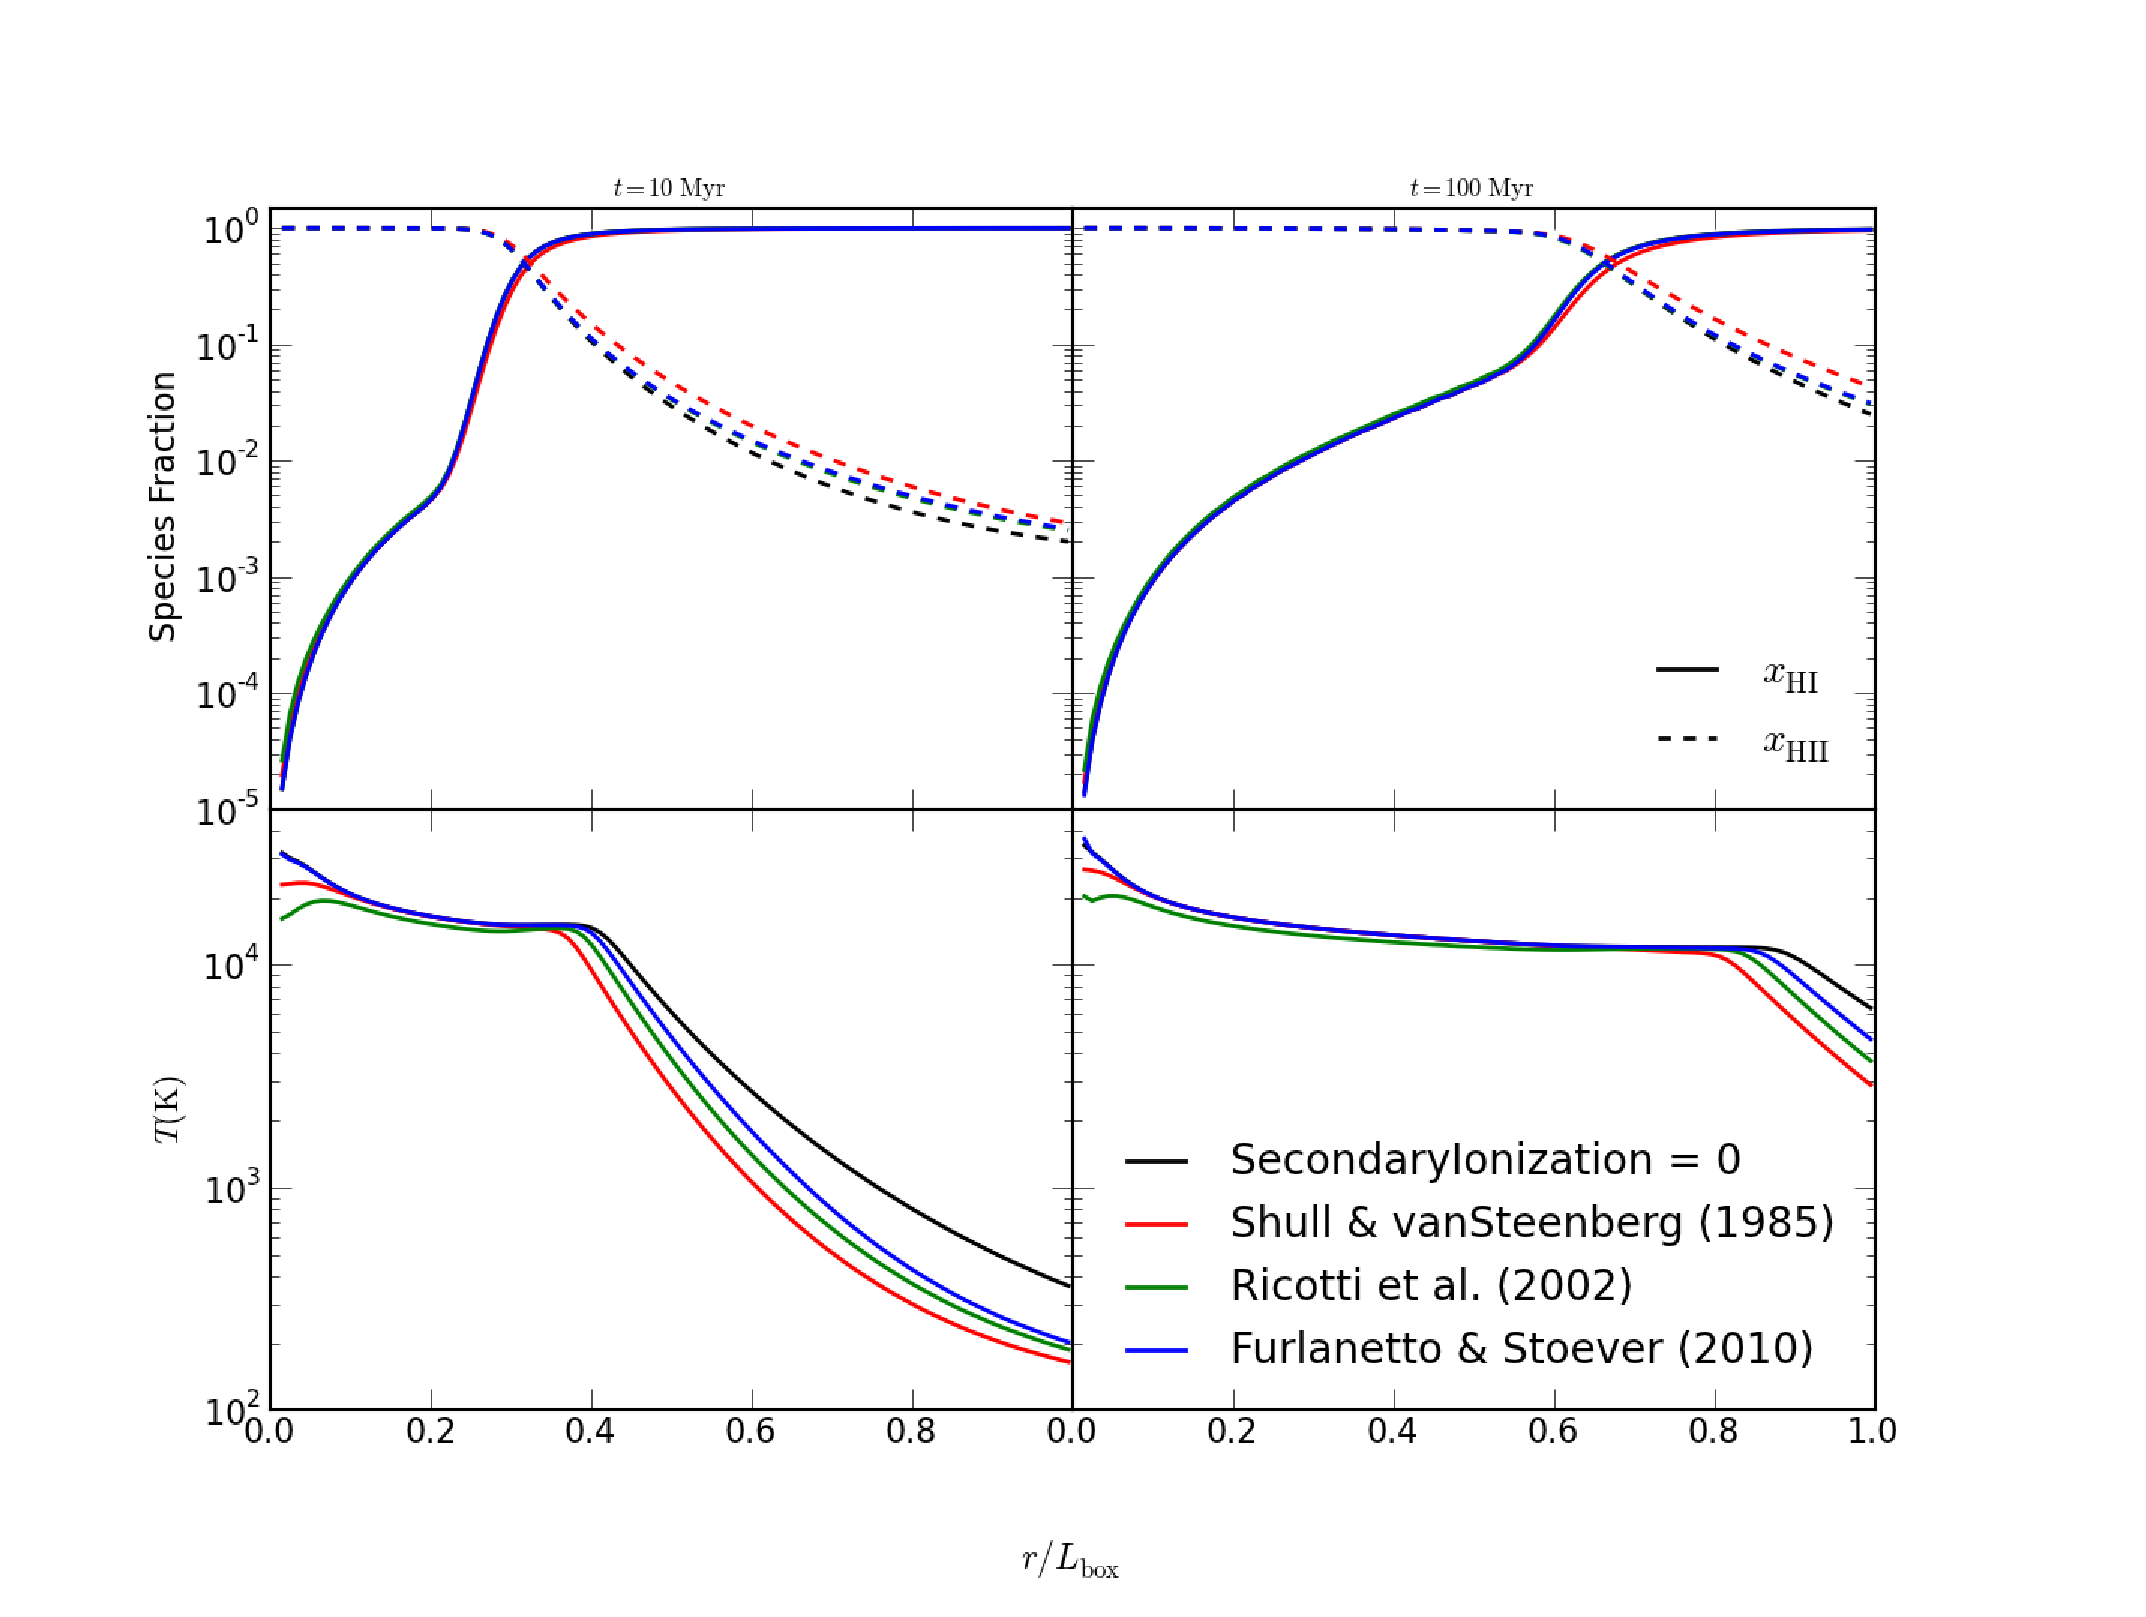
\includegraphics[width=0.98\textwidth]{figures/secondary_ionization_methods.eps}
\caption{Comparison of different methods for secondary ionization.  See \S\ref{sec:PhysicsParameters} for details on setting the secondary ionization method.}
\label{fig:SecondaryIonizationMethods}
\end{center}
\end{figure*}

\subsection{Time-stepping Techniques}



\subsection{Parallelism}

%%% 
%% Classes
%%%
\section{Classes}
In order of appearance in \texttt{RT1D.py}.

\subsection{\texttt{InitializeGrid}}
Initialize the temperature and ion densities for each cell in the grid.
\subsection{\texttt{InitializeIntegralTables}}
If \texttt{IntegralTabulation} = 1 (necessary when \texttt{DiscreteSpectrum} = 0), tabulates the quantities $\Phi_i$ and $\Psi_i$.  If \texttt{MultiSpecies} = 1, tabulation occurs for hydrogen and helium ions, and if \texttt{SecondaryIonization} $\ge 2$, also tabulate $\widetilde{\Phi}_i$, $\widetilde{\Psi}_i$, $\widehat{\Phi}_i$, and $\widehat{\Psi}_i$, adding an additional dimension for $x_{\mathrm{HII}}$.
\subsection{\texttt{RadiationSource}}
Initialize the radiation source.  Most importantly the \texttt{Spectrum} function, which returns the fraction of the bolometric luminosity emitted at energy $E$ (only argument).
\subsection{\texttt{Radiate}}
Calls \texttt{EvolvePhotons} routines, which loop over grid, call solver, and update ion densities and the temperature in each cell.
\subsection{\texttt{SolveRateEquations}}
ODE solver.
\subsection{\texttt{Interpolate}}
Performs linear, bi-linear, tri-linear, and eventually quad-linear interpolation on integral tables to extract ionization and heating coefficients as a function of column density.
\subsection{\texttt{WriteData}}
Write out data to HDF5.  Would be easy to add support for ASCII write-out.

%%% 
%% Parameters
%%%
\section{Parameters} \label{sec:Parameters}

\subsection{Problem Types}
These were added for convenience in January, 2011.  If you want to make changes to these test problems you can, just make sure \texttt{ProblemType} is the first (uncommented) line in your parameter file.  Additional parameters afterwards will be interpreted as usual.

\begin{description}
    
\item [\texttt{ProblemType = 1}] This will set up a standard test with known analytic solution: the propagation of an ionization front in an isothermal, hydrogen-only, static universe.  The spectrum used is monochromatic at $E = 13.6 \ \text{eV}$, with photon luminosity $L_{\nu} = 5\times 10^{48} \ s^{-1}$.  The initial density, temperature, and box size are the same as the values used in Test 1 of Wise \& Abel 2010. 

\item [\texttt{ProblemType = 2}] This problem is almost exactly the same as \texttt{ProblemType = 1}.  However, the temperature is allowed to evolve, and instead of using a monochromatic spectrum, we use a $10^5$ K blackbody spectrum.  Again, the initial density, temperature, box size, and energy groups are the same as the values used in Test 1 of Wise \& Abel 2010.  

\item [\texttt{ProblemType = 2.1}] Same as \texttt{ProblemType = 2}, except we sample the continuous blackbody spectrum with the four energy groups used by \citet{Wise2011}.

\item [\texttt{ProblemType = 2.2}] Same as \texttt{ProblemType = 2}, except we sample the continuous blackbody spectrum with the four energy groups used by Mirocha et al. (2012).

\item [\texttt{ProblemType = 3}] Test problem \# 3 from \cite{Iliev2006} -- I-front trapping in a dense clump and the formation of a shadow.  The setup is the same as in \texttt{ProblemType = 2}, except a 1D clump is initialized at $x = 0.76 L_{\mathrm{box}}$, overdensity $\delta = 200$, radius $0.12$kpc, and temperature $T = 40$K, and the radiation field is plane-parallel.

\item [\texttt{ProblemType = 3.1}] Same as \texttt{ProblemType = 3}, except we sample the continuous blackbody spectrum with the four energy groups used by \citet{Wise2011}.

\end{description}

\subsection{Initial Conditions}
\begin{description}
    
\item [\texttt{DensityProfile}]  

\item [\texttt{TemperatureProfile}]

\item [\texttt{InitialHIIFraction}]  

\end{description}


\subsection{Control Parameters}

\begin{description}
    
\item [\texttt{ODEatol}] Absolute tolerance of the ODE solver.  If ionized fractions are zero to this tolerance, they are reset to \texttt{MinimumSpeciesFraction}.  Combination of this parameter and \texttt{ODErtol} (below) determine whether or not the ODE time-step is cut in half. (Default = $10^{-5}$)

\item [\texttt{ODErtol}]
Relative tolerance of the ODE solver.  Combination of this parameter and \texttt{ODEatol} determine whether or not the ODE time-step is cut in half via the formulae $|y_2 - y_1| = \texttt{ODEatol} + \texttt{ODErtol}\times y_2$. (Default = $10^{-5}$)
 

\end{description}


\subsection{Source Parameters}


\subsection{Physics Parameters} \label{sec:PhysicsParameters}


\section{Analysis}
Since our datasets are small, we can read in the entire time evolution all at once.  To do this, type the following in a Python terminal:
\begin{verbatim}
import rt1d.analysis as rta
import pylab as pl

ds = rta.Analyze('./pf.dat')                # load parameter file and data
pl.loglog(ds.data[10].r, ds.data[10].x_HI)  # radius vs. neutral fraction
\end{verbatim}

%%%
%% Test Problems
%%%
\section{Test Problems}
In this section we focus on test problems 1-3 of the Radiative Transfer Comparison Project \citep[hereafter RT06;][]{Iliev2006}.

\subsection{Test \#0}
Single-zone ionization, heating, and cooling.

\begin{figure*}[htbp!]
\begin{center}
\includegraphics[width=0.98\textwidth]{figures/rt06_0.eps}
\caption{Convergence test for RT06 \#1.}
\label{fig:RT06_1}
\end{center}
\end{figure*}

\subsection{Test \#1}

\begin{figure*}[htbp!]
\begin{center}
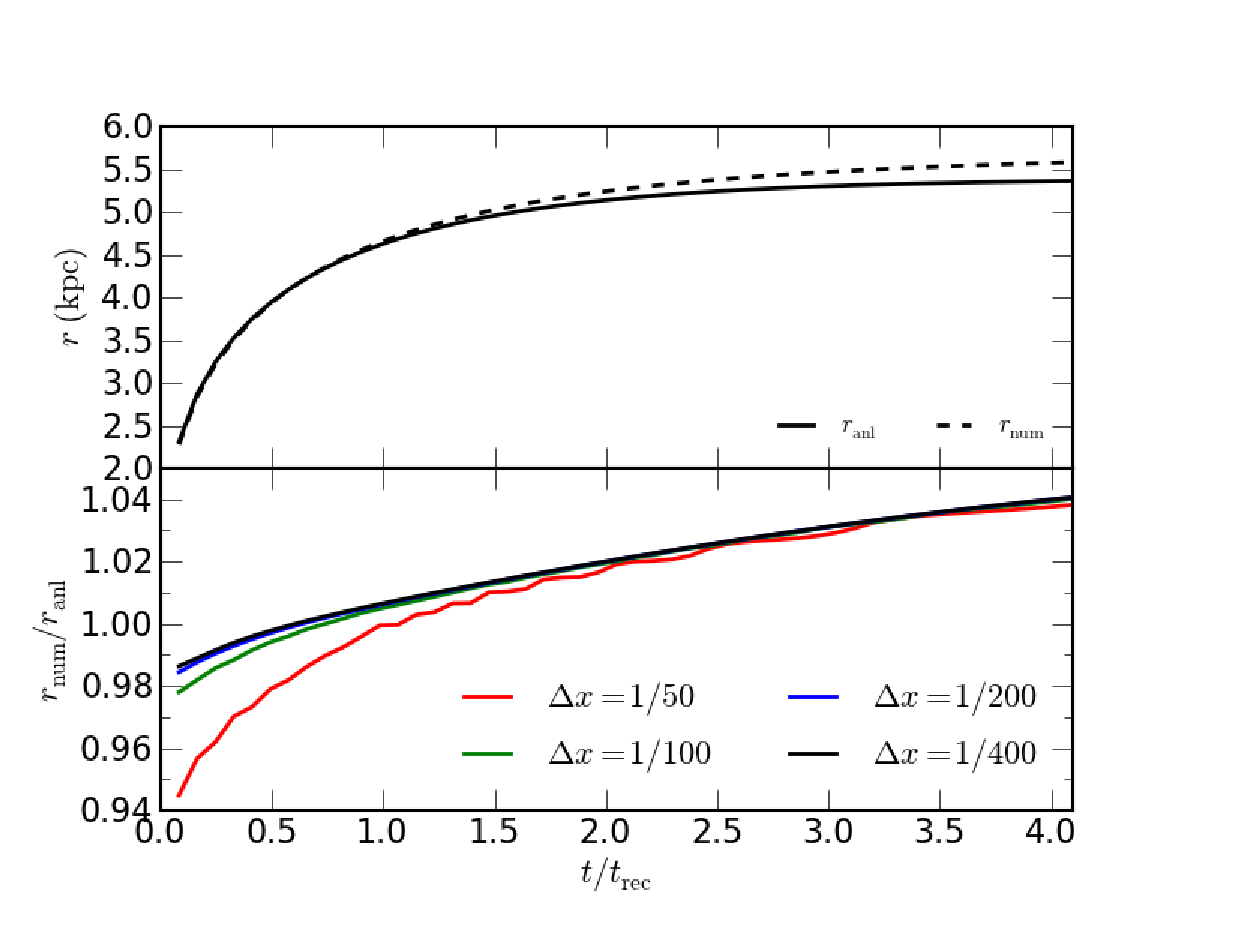
\includegraphics[width=0.98\textwidth]{figures/rt06_1_convergence.eps}
\caption{Convergence test for RT06 \#1.}
\label{fig:RT06_1}
\end{center}
\end{figure*}

\subsection{Test \#2}

\begin{figure*}[htbp!]
\begin{center}
\includegraphics[width=0.98\textwidth]{figures/rt06_2.eps}
\caption{RT06 \#3.}
\label{fig:RT06_2}
\end{center}
\end{figure*}
            
\subsection{Test \#3}

\begin{figure*}[htbp!]
\begin{center}
\includegraphics[width=0.98\textwidth]{figures/rt06_3.eps}
\caption{RT06 \#3.}
\label{fig:RT06_3}
\end{center}
\end{figure*}

%%% 
%% Start to Finish
%%%
\section{Start to Finish}

%%% 
%% Convergence
%%%
\section{Convergence}
In \texttt{rt1d/doc/examples} you will find directories containing convergence test suites for RT06 test problems 1 \& 2 (\texttt{RT06\_1\_ResolutionTestSuite} and \texttt{RT06\_2\_ResolutionTestSuite}).  Each of these directories contains the parameter files necessary to run these problems on grids containing $100 \times 2^n$ cells, where $n = 0,1,...6$.  If you want, you can run them all at once, though keep in mind the simulations with 100 cells will finish much much faster than those containing 6400 cells, so it might not be good to check out a node for this as most of the computation will be spent on 1 or 2 simulations.  For instance, you could do:
\begin{verbatim}
    cd rt1d/doc/examples/RT06_1_ResolutionTestSuite/c_infinite
    mpirun -np 4 python RT1D.py -b batch_list.dat
\end{verbatim}
I've included the same setup for $c \neq \infty$ in \texttt{rt1d/doc/examples/RT06\_1\_ResolutionTestSuite/c\_finite}, so you can see the differences (if any) caused by making the $c \rightarrow \infty$ approximation.

%%% 
%% Troubleshooting
%%%
\section{Troubleshooting}
If your results look horribly, horribly wrong, here are a few places where you could've gone wrong.  We'll start with things that may occur with the stable version of the code.


Now, if you modify or add anything in the source code (awesome by the way!), you're far more likely to encounter troubles.


\begin{description}
    \item[Totally Bogus Results] This is will almost certainly happen at some point in the development process. But, if it happens even after you're \textit{positive} the error was fixed, my guess is that you are using the integral tables that were generated with the previous, error-ridden version of the code.  Try removing the integral tables and re-running your simulation.
\end{description}

%%%
%% INTERACTIVE MODE
%%%
\section{Interactive Mode}
Is it worth doing this?  Would want it to look something like this:

\begin{verbatim}
import rt1d
import numpy as np
pf = rt1d.SetDefaultParameterValues()
r = np.linspace(3e19, 3e21, 100) # 100 grid cells between 0.01-1kpc. (optional)
data = rt1d.Shine(pf, r)    
\end{verbatim}    

This would make it easy to:
\begin{itemize}
    \item Allow users to write their own rt1d `scripts.'
    \item Change source properties manually with time.
    \item Making arbitrarily structured grids.
    \item Very specific initial conditions.
\end{itemize}    

What parameters must be set?
\begin{itemize}
    \item ProblemType
    \item GridDimensions
    \item MultiSpecies
    \item LengthUnits
    \item InitialDensity
    \item SourceParameters
\end{itemize}

\newpage
\bibliography{references}
\bibliographystyle{apj}





\end{document}



